\documentclass{article}
\usepackage[letterpaper,top=2cm,bottom=2cm,left=3cm,right=3cm,marginparwidth=1.75cm]{geometry}
\usepackage{amsmath}
\usepackage{graphicx}
\usepackage{fancyhdr}
\renewcommand{\footrulewidth}{1pt}
\fancyfoot[L]{\leftmark}
\fancyfoot[C]{\textbf{n° \thepage}} 
\fancyfoot[R]{15.11.2024}
\usepackage{colortbl}
\usepackage{multirow}
\usepackage{booktabs}
\usepackage{hhline}
\usepackage{amsmath}
\usepackage{amsfonts}
\usepackage{graphicx}
\usepackage{subcaption}
\usepackage{float}
\usepackage{array}
\usepackage{listings}
% \usepackage{subcaption}
\usepackage{appendix}
\usepackage{pgfplotstable}
\pgfplotsset{compat=1.18}


\usepackage{siunitx}

\usepackage{booktabs} % For better table formatting

\usepackage{amsthm}
\usepackage{amssymb}
\usepackage{enumitem}


\usepackage[hidelinks]{hyperref}
% \usepackage{hyperref}


\usepackage{cleveref}

\usepackage{multirow}
\usepackage{tabularx}

%Definitions
%\theoremstyle{definition}
\newtheorem{df}{Definition}[section]
\newtheorem{problem}{Problem}[section]
\newtheorem{remark}{Remark}[section]
\newtheorem{ex}{Example}[section]
%Theorems and Lemmas
\newtheorem{thm}{Theorem}[section]
\newtheorem{corollary}{Corollary}[thm]
\newtheorem{lemma}[thm]{Lemma}
\newtheorem{prop}[thm]{Proposition}

% Adjust spacing above and below displayed equations
\usepackage{setspace}
\setdisplayskipstretch{1.3}
\setlength{\jot}{8pt} 


% Customize lstlistins captions
\newcommand{\codeexcerptname}{Fragment}
\usepackage{caption}
\DeclareCaptionFormat{mylistings}{#1#2#3}
% \captionsetup[lstlisting]{format=mylistings, labelsep=space} % Remove colon
\renewcommand\lstlistingname{\codeexcerptname} % Custom name for lstlistings

% Rename Cref link to code fragments
\Crefname{listing}{\codeexcerptname}{\codeexcerptname s}

% Usage: \codeListing{FIILE.py}{FIRSTLINE}{LASTLINE}{CAPTION}{LABEL}
\newcommand{\codeListing}[5]{%
    \lstinputlisting[
      language=Python,
      caption={\href{https://gitlab.epfl.ch/jfox/optimization-on-manifolds-project-1/-/blame/main/code/#1?ref_type=heads\#L#2}{(\texttt{\detokenize{#1}})}: #4},
      firstline=#2,
      lastline=#3,
      firstnumber=#2,
      label={#5}]{code/#1}%
}


% Macros
\newcommand{\argwrap}[1]{\left(#1\right)}
\newcommand{\argwrapsquare}[1]{\left[#1\right]}
\newcommand{\intS}[1]{\ensuremath{\int_{\Omega}#1 \, dS}}
\newcommand{\intSlong}[1]{\intS{\argwrapsquare{#1}}}
\newcommand{\darg}[2]{\ensuremath{\, \partial_{#2}#1} \, }
\newcommand{\dt}[1]{\ensuremath{\darg{#1}{t}}}
\newcommand{\dS}[1]{\ensuremath{\darg{#1}{S}}}
\newcommand{\dSlong}[1]{\darg{\argwrap{#1}}{S}}
\newcommand{\dSS}[1]{\ensuremath{\darg{#1}{SS}}}
\newcommand{\dtu}{\dt{u}}
\newcommand{\dSu}{\dS{u}}
\newcommand{\dSSu}{\dSS{u}}
\newcommand{\dtv}{\dt{v}}
\newcommand{\dSv}{\dS{v}}
\newcommand{\dSSv}{\dSS{v}}
\newcommand{\sigmafrac}{\ensuremath{\frac{\sigma^2}{2}}}
\newcommand{\czero}{\ensuremath{C^0((0,T];L^2(\Omega))}}
\newcommand{\seminorm}[1]{\ensuremath{|#1|_V}}
\newcommand{\norm}[1]{\ensuremath{\|#1\|_{L^2(\Omega)}}}
\newcommand{\seminormsq}[1]{\ensuremath{|#1|_V^2}}
\newcommand{\normsq}[1]{\ensuremath{\|#1\|_{L^2(\Omega)}^2}}
\newcommand{\aform}[2]{\ensuremath{\sigmafrac \intS{S^2 \dS{#2} \dS{#1}} + (\sigma^2 - r) \intS{S #2 \dS{#1}} + \intS{r  #1  #2}}}
\newcommand{\auv}{\aform{u}{v}}









\begin{document}

\thispagestyle{empty}

\begin{figure}
\centering

\includegraphics[width=0.5\textwidth]{code/images/LOGO.png}
\end{figure}
\vspace{0.5cm}
\begin{center}
\textsc{ \Large MATH-451: Numerical Approximation of PDEs}
\vspace{1.5cm}
\hrule
\vspace{0.5cm}
{\huge \bfseries Black-Scholes Equation: European Put}
\vspace{0.5cm}
\hrule
\vspace{1.5cm}


\emph{\Large \centering Author:}\\
\vspace{0.3cm}

\large Mattia \textsc{\large Barbiere} (387974)\\

~

\vspace{0.5cm}


\emph{\Large \centering Professor:}\\
\vspace{0.3cm}
\large  Annalisa  \textsc{\large Buffa}\\
~

\vspace{0.5cm}

\large Spring Semester - 2025

\end{center}

\clearpage
\pagenumbering{arabic}

Let us define the following quantities
\begin{problem}[Black \& Scholes Equation for European Put Option]\label{def:problem}
Consider the Black \& Scholes equation for the value \( u(S, t) \) of an European Put option:
\[
\begin{cases}
\partial_t u - \frac{\sigma^2}{2} S^2 \partial_{SS} u - r S \partial_S u + r u = 0 & \text{in } \Omega \times (0, T], \\
u(S, 0) = u_0(S) = \max \{ K - S, 0 \},
\end{cases}
\]
where \(\Omega = (S_{\min}, S_{\max})\), \(\sigma\) and \(r\) are strictly positive and bounded constants, together with the following boundary conditions:
\[
\partial_S u(S_{\min}, t) = u(S_{\max}, t) = 0.
\]
\end{problem}

\begin{df}[Weighted Sobolev Space]
We introduce the weighted Sobolev space \( V \):
\[
V = \left\{ v : v \in L^2(\Omega), S \frac{\partial v}{\partial S} \in L^2(\Omega), v(S_{\max}) = 0 \right\}.
\]
Endowed with the inner product and norm:
\[
(v, w)_V = \int_\Omega \left( v(S) w(S) + S^2 \frac{\partial v}{\partial S}(S) \frac{\partial w}{\partial S}(S) \right) dS, \quad \| v \|_V = (v, v)_V^{1/2}.
\]
The seminorm
\[
|v|_V^2 = \int_\Omega \left( S \frac{\partial v}{\partial S} \right)^2 dS
\]
is a norm in the Hilbert space \( V \) and we have the following Poincaré inequality:
\[
\| v \|_{L^2(\Omega)} \leq 2 |v|_V, \quad \forall v \in V.
\]
\end{df}

\section{Question A}
\begin{df}\label{def:a}
    For $u \in \czero$ and $v \in V$ we define the following bilinear form
    \begin{equation*}
        a(u,v) := \auv
    \end{equation*}
\end{df}
\begin{prop}\label{prop:variational_form}
    The variational form of the problem defined in \Cref{def:problem} is
    \begin{align*}
    &\left( \dtu, v\right) + a(u,v) = \\
    &= \intS{v \dtu} + \auv = 0
    \end{align*}
\end{prop}
\begin{proof}
    Take $v \in V$. Starting from \Cref{def:problem} we multiply by the test function $v$ and integrate over $\Omega$,
    \begin{equation*}
        \intS{v \dtu} - \intS{\sigmafrac S^2  v  \dSSu } - \intS{r S v \dSu} + \intS{r  u  v} = 0.
    \end{equation*}
    We now apply \Cref{thm:by_parts} to the second term. Thus we are left with
    \begin{equation*}
        \intS{v \dtu} - \sigmafrac \left[ \left. \left[S^2 v \dSu \right] \right|_{\partial\Omega} - \intS{\dS{(S^2v)} \dSu}\right] - \intS{r S v \dSu} + \intS{r  u  v} = 0.
    \end{equation*}
    On the boundary we have that
    \begin{align*}
        (S_{min})^2 v(S_{min}) \dSu(S_{min}, t) &= 0 \text{ because of the boundary condition } \dSu(S_{min}, t) = 0\\
        (S_{max})^2 v(S_{max}) \dSu(S_{max}, t) &= 0 \text{ because of the boundary condition } v(S_{max}) = 0
    \end{align*}
    allowing us to eliminate the boundary term. Next using the product rule of the differential gives 
    \begin{equation*}
        \intS{v \dtu} + \sigmafrac \intSlong{2Sv \dSu + S^2 \dSv \dSu} - \intS{r S v \dSu} + \intS{r  u  v} = 0.
    \end{equation*}
    Next using the inner product $\left( \dtu, v\right) = \intS{v \dtu}$ and \Cref{def:a} we can rewrite this as
    \begin{align*}
    &\left( \dtu, v\right) + a(u,v) = \\
    &= \intS{v \dtu} + \auv = 0 \qedhere
    \end{align*}
    \end{proof}

\begin{prop}\label{prop:ineq_a}
    For any $t \in (0,T]$ and any $v \in V$ we have that
    \begin{equation*}
        a(v,v) \geq \frac{\sigma^2}{4} \seminorm{v} - \alpha \normsq{v}
    \end{equation*}
    where $\alpha > 0$ is defined as
    \begin{equation*}
        \alpha = \begin{cases}
            \frac{(\sigma^2 - r)^2}{ \sigma^2}, &\text{ if } \quad r \neq \sigma^2\\
            \varepsilon, &\text{ if } \quad r = \sigma^2\\
        \end{cases}
    \end{equation*}
    with $\varepsilon$ being any positive real number. In particular, $\varepsilon >0$ can be chosen arbitrarily small.
    \begin{proof}
        Recalling \Cref{def:a} we have that
        \begin{align*}
            a(v,v) &= \aform{v}{v}.
        \end{align*}
        By definition of $\normsq{\cdot}$ and $\seminormsq{\cdot}$ we have that
        \begin{equation*}
            a(v,v) = \sigmafrac \seminormsq{v} + (\sigma^2 - r) \intS{S v \dSv} + r \normsq{v}.
        \end{equation*}
        Using properties of the absolute value we can bound this by below
        \begin{equation}\label{eq:first_lower_bound_a}
            a(v,v) \geq \sigmafrac \seminormsq{v} - \left| (\sigma^2 - r) \intS{S v \dSv}\right| + r \normsq{v}.
        \end{equation}
        Let us focus on bounding the second term
        \begin{align*}
            - \left| (\sigma^2 - r) \intS{S v \dSv}\right| &\geq - \left| (\sigma^2 - r) \right| \intS{\left|S v \dSv \right|} && \text{ by the triangle inequality}\\
            &\geq -\left| (\sigma^2 - r) \right| \norm{S \dSv} \norm{v} && \text{ by Cauchy–Schwarz inequality}\\
            &\geq -\left| (\sigma^2 - r) \right| \left( \frac{ \normsq{S \dSv}}{2 \delta} + \frac{\delta \normsq{v}}{2}\right) && \text{ by Young's inequality, $\delta >0$}\\
            & \geq - \frac{\sigma^2}{4} \seminormsq{v} - \frac{(\sigma^2 - r)^2 \normsq{v}}{ \sigma^2}
        \end{align*}
        where the last inequality came from choosing $\delta = 2| (\sigma^2 - r) | / \sigma^2$. Plugging this back into \Cref{eq:first_lower_bound_a} give us the following lower bound for $a(v,v)$
        \begin{align*}
            a(v,v) &\geq \frac{\sigma^2}{4} \seminormsq{v} - \frac{(\sigma^2 - r)^2}{ \sigma^2} \normsq{v} + r \normsq{v}\\
            &\geq \frac{\sigma^2}{4} \seminormsq{v} - \frac{(\sigma^2 - r)^2}{ \sigma^2} \normsq{v}.
        \end{align*}
        by noticing that $r \normsq{v} \geq 0$.
        
        Let us now consider two cases. Firstly, if $r \neq \sigma^2$ we can choose $\alpha = (\sigma^2 - r)^2 / \sigma^2 > 0$ and get
        \begin{equation*}
            a(v,v) \geq \frac{\sigma^2}{4} \seminormsq{v} - \alpha \normsq{v}
        \end{equation*}
        which is the desired inequality.

        Secondly if $r = \sigma^2$ we can choose any $\alpha >0$ and, in particular, we can choose $\alpha$ arbitrarily close to $0$. For whatever choice of $\alpha > 0$ the following holds
        \begin{equation*}
            a(v,v) \geq \frac{\sigma^2}{4} \seminormsq{v} - \alpha \normsq{v}
        \end{equation*}
        which is again the requested inequality.
    \end{proof}
\end{prop}

\section{Question B}
Before answering this question I present a useful algebraic identity
\begin{lemma}\label{lemma_alg_id_and_ineq}
    For any integrable functions $f, g$ we have that
    \begin{equation*}
        \intS{(f - g)f} = \frac{1}{2}\left( \normsq{f} - \normsq{g} + \normsq{f - g}\right).
    \end{equation*}
    Moreover,
    $$\intS{(f - g)f} \geq \frac{1}{2}\left( \normsq{f} - \normsq{g} \right)$$
\end{lemma}
\begin{proof}
    Starting from the right hand side we have that
    \begin{align*}
        &\frac{1}{2}\left( \normsq{f} - \normsq{g} + \normsq{f - g}\right) =\\
        &=\frac{1}{2}\left(\intS{f^2} -  \intS{g^2} + \intS{f^2} +  \intS{g^2} - 2\intS{fg} \right) =\\
        &=\intS{f^2} - \intS{fg} = \intS{(f - g)f}.
    \end{align*}
    The second part is immediate after noticing that $\normsq{f - g} \geq 0$.
\end{proof}

\begin{lemma}\label{lemma:semi_discrete_prob}
    A semi-discretization of the problem defined in \Cref{def:problem} is the following
     \begin{align*}
        &\intSlong{\frac{u^{j} - u^{j-1}}{\Delta t}  v} + \\
        &+\sigmafrac \intS{S^2 \left(\dS{\left(\theta u^{j} + (1- \theta) u^{j-1} \right)}\right) \dSv} + \\
        &+ (\sigma^2 - r) \intS{S v \dS{\left(\theta u^{j} + (1- \theta) u^{j-1} \right)}} + \\
        &+r \intS{\left(\theta u^{j} + (1- \theta) u^{j-1} \right)v} =\\
        &=0.
        \end{align*}
\end{lemma}
\begin{proof}
    Recall the variational form of the problem as shown in \Cref{prop:variational_form}
    \begin{align*}
        &\left( \dtu, v\right) + a(u,v) = \\
        &= \intS{v \dtu} + \auv = 0.
    \end{align*}
    We aim to discretize in time only. Using finite difference for approximating the derivative and replacing $u$ with $\theta u^{j} + (1- \theta) u^{j-1}$
     \begin{align*}
        &\intSlong{\frac{u^{j} - u^{j-1}}{\Delta t}  v} + \\
        &+\sigmafrac \intS{S^2 \left(\dS{\left(\theta u^{j} + (1- \theta) u^{j-1} \right)}\right) \dSv} + \\
        &+ (\sigma^2 - r) \intS{S v \dS{\left(\theta u^{j} + (1- \theta) u^{j-1} \right)}} + \\
        &+r \intS{\left(\theta u^{j} + (1- \theta) u^{j-1} \right)v} =\\
        &=0.
        \end{align*}
\end{proof}
Before answering the question I introduce some useful definition and lemmas.


\begin{df}\label{def:b}
    For $v,w \in V$ and $\Delta t \in \mathbb{R}$ define the bilinear form $b(v, w)$ as
    \begin{equation*}
        b(v, w) := \intS{v\,w} + \Delta t\,a(v,w)
    \end{equation*}
\end{df}

\begin{lemma}\label{lemma:b_lax_assump}
    Assume $\Delta t \leq \frac{1}{2\alpha}$ where $\alpha$ is defined in \Cref{prop:ineq_a}. Then for any $v,w \in V$ the bilinear form $b(\cdot, \cdot)$ defined in \Cref{def:b} satisfies
    \begin{align*}
        & b(v,w) \leq M \| v\|_V \| w\|_V \quad \text{ (Continuity) }\\
        &b(v,v) \geq \beta \| v\|_V^2 \qquad \hspace{6mm} \text{ (Coercivity) }
    \end{align*}
    for some $M,\beta>0$.
\end{lemma}
\begin{proof}
    By definition of $b(v, w)$ we have that
    \begin{align*}
        b(v,w) &= \intS{v\,w} + \Delta t\,a(v,w)\\
        &= \intS{v\,w} + \aform{v}{w}.
    \end{align*}
    Using Hölder's inequality multiply times and the definition of the seminorm, this can all be bounded by
    \begin{align*}
        b(v,w)  &\leq \normsq{v}\normsq{w} + \sigmafrac\seminormsq{v}\seminormsq{w} + (\sigma^2 - r ) \seminormsq{v}\normsq{w} + r \normsq{v} \normsq{w}\\
        &\leq (1+r)\normsq{v} \normsq{w}+ \sigmafrac\seminormsq{v}\seminormsq{w} + \left|\sigma^2 - r\right| \seminormsq{v}\normsq{w}.
    \end{align*}
    As $v,w \in V$, by the definition of the space $V$ we have that $\seminormsq{v}, \seminormsq{w} < + \infty$ thus, as the above equation is finite, there must exist an $M >0$ such that
    \begin{equation*}
        b(v,w)  \leq M \| v\|_V \| w\|_V.
    \end{equation*}
    For coercivity $b(v, v)$ can be bounded by below by
    \begin{align*}
        b(v, v) &= \normsq{v} + \Delta t\, a(v,v) \geq \normsq{v} + \Delta t\, a(v,v)\\
        & \geq \normsq{v} + \Delta t\, \left( \frac{\sigma^2}{4} \seminormsq{v} - \alpha \normsq{v} \right) \\
        &= \left(1 - \Delta t \, \alpha  \right) \normsq{v} +\Delta t\, \frac{\sigma^2}{4} \seminormsq{v}
    \end{align*}
    where the second inequality comes \Cref{prop:ineq_a}. By assumption we have that $\Delta t \leq \frac{1}{2\alpha}$ and hence $\left(1 - \Delta t \, \alpha  \right) \geq \frac{1}{2}$ giving
    \begin{align*}
        b(v, v) &\geq \frac{1}{2}\normsq{v} +\Delta t\, \frac{\sigma^2}{4} \seminormsq{v}\\
        & \geq \min\left(\frac{1}{2}, \Delta t\,\frac{\sigma^2}{4}\right) \left( \normsq{v} +  \seminormsq{v}\right)\\
        &= \beta \| v\|_V^2
    \end{align*}
    by taking $\beta = \min\left(\frac{1}{2}, \Delta t\,\frac{\sigma^2}{4}\right) > 0$. \qedhere
\end{proof}

\begin{prop}\label{prop:lax_milgram}
    The semi-discrete problem in \Cref{lemma:semi_discrete_prob} with $\theta = 1$ is well posed for any time step $\Delta t \leq \frac{1}{2 \alpha}$.
\end{prop}
\begin{proof}
    Using $\theta = 1$ in the result of \Cref{lemma:semi_discrete_prob} leaves us with
    \begin{align*}
        &\intSlong{\frac{u^{j} - u^{j-1}}{\Delta t}  v} +\sigmafrac \intS{S^2 \dS{\left(u^{j}\right)} \dSv} + (\sigma^2 - r) \intS{S v \dS{\left(u^{j}\right)}} + r \intS{u^{j}v} =0.
        \end{align*}
    Using \Cref{def:a} we can simplify this as
    \begin{equation*}
    \intSlong{\frac{u^{j} - u^{j-1}}{\Delta t} v} + a(u^{j},v) = 0.
    \end{equation*}
    Moving terms around
    \begin{equation*}
        \intS{u^{j}v} + \Delta t \,a(u^{j},v) = \intS{u^{j-1}v}.
    \end{equation*}
    We now perform induction over $j$ to prove that the problem is well posed.\\
    \textbf{Base case:} $j = 1$. In this case
    \begin{equation*}
        \intS{u^{1}v} + \Delta t \,a(u^{1},v) = \intS{u^{0}v}.
    \end{equation*}
    and as $u^0$ is known and thus this is equivalent to 
    \begin{equation}\label{eq:base_case}
        b(u^{1}, v) = F(v)
    \end{equation}
    by \Cref{def:b}. Invoking the Lax-Milgram Lemma \Cref{lemma:lax_mil} and \Cref{lemma:b_lax_assump} we conclude that there exists a unique $u^1$ solving \Cref{eq:base_case}.\\
    \textbf{Induction case: } For a general value of $j$ we have, assume that for $j-1$ the problem is well posed. Then this implies that $u^{j-1}$ exists and is unique. For this reason we can write the problem as
    \begin{equation*}
        b(u^{j},v)=\intS{u^{j}v} + \Delta t \,a(u^{j},v) = \intS{u^{j-1}v} = F(v)
    \end{equation*}
    and as $u^{j-1}$ is fixed. The conclusion comes once again by the Lax-Milgram Lemma \Cref{lemma:lax_mil} and \Cref{lemma:b_lax_assump}, proving that the problem is well posed for all $j$. \qedhere
    
    
\end{proof}

\begin{prop}
    Given the semi-discrete problem in \Cref{lemma:semi_discrete_prob} with $\theta = 1$ (i.e implicit Euler), for any time step $\Delta t \leq \frac{1}{2 \alpha}$ the following inequality holds\\
    \begin{equation*}
        (1 - 2\alpha \Delta t)^N \| u^N \|_{L^2}^2 + \frac{\Delta t}{2} \sigma^2 \sum_{j=1}^{N-1} (1 - 2\alpha \Delta t)^{j-1} \seminormsq{u^j} \leq \| u^0 \|_{L^2}^2.
        \label{eq:placeholder_label}
    \end{equation*}
\end{prop}
\begin{proof}
    Using $\theta = 1$ and $v = u^j$ in the result of \Cref{lemma:semi_discrete_prob} leaves us with
    \begin{align*}
        &\intSlong{\frac{u^{j} - u^{j-1}}{\Delta t}  u^{j}} +\sigmafrac \intS{S^2 \dS{\left(u^{j}\right)} \dS{u^{j}}} + (\sigma^2 - r) \intS{S u^{j} \dS{\left(u^{j}\right)}} + r \intS{(u^{j})^2} =0.
        \end{align*}
    which can be rewritten as
    \begin{equation}\label{eq:discret_time_and_a_u_j+1}
        \intSlong{\frac{u^{j} - u^{j-1}}{\Delta t}  u^{j}} + a(u^{j},u^{j}) = 0.
    \end{equation}
   We start by multiplying \Cref{eq:discret_time_and_a_u_j+1} by $\Delta t \geq 0$
   \begin{equation*}
    \intSlong{(u^{j} - u^{j-1})  u^{j}} + \Delta t \,a(u^{j},u^{j}) = 0.
    \end{equation*}
    Next we use the inequality in \Cref{lemma_alg_id_and_ineq} using $f = u^{j}$ and $g =u^{j-1}$
    \begin{equation*}
        \frac{1}{2}\left( \normsq{u^{j+1}} - \normsq{u^{j}} \right) + \Delta t \,a(u^{j+1},u^{j+1}) \leq 0.
    \end{equation*}
    After multiplying by $2$ we can invoke \Cref{prop:ineq_a} and we are left with
    \begin{equation*}
         \normsq{u^{j}} - \normsq{u^{j-1}} + 2\Delta t \, \left( \frac{\sigma^2}{4} \seminormsq{u^{j}} - \alpha \normsq{u^{j}} \right) \leq 0.
    \end{equation*}
    After moving some terms around this can be rewritten as
    \begin{equation*}
        (1- 2\alpha \Delta t)\normsq{u^{j}}  - \normsq{u^{j-1}} + \Delta t \, \sigmafrac \seminormsq{u^{j}} \leq 0.
    \end{equation*}
   We multiply everything by $(1- 2\alpha \Delta t)^{j-1}$
   \begin{equation*}
       (1- 2\alpha \Delta t)^{j}\normsq{u^{j}}  - (1- 2\alpha \Delta t)^{j-1} \normsq{u^{j-1}} + \Delta t \, \sigmafrac (1- 2\alpha \Delta t)^{j-1}\seminormsq{u^{j}} \leq 0.
   \end{equation*}
   As this inequality is valid for all $j \in \{1, \ldots, N \}$ we can take the sum over $j$ and we observe that the first two terms form a telescoping sum
   \begin{align*}
       &\sum_{j=1}^{N} \left[(1- 2\alpha \Delta t)^{j}\normsq{u^{j}}  - (1- 2\alpha \Delta t)^{j-1} \normsq{u^{j-1}}\right] + \Delta t \, \sigmafrac \sum_{j=1}^{N}(1- 2\alpha \Delta t)^{j-1}\seminormsq{u^{j}} \\
       &\leq (1- 2\alpha \Delta t)^{N}\normsq{u^{N}} - \normsq{u^{0}} + \Delta t \, \sigmafrac \sum_{j=1}^{N}(1- 2\alpha \Delta t)^{j-1}\seminormsq{u^{j}} \leq 0.
   \end{align*}
   We conclude by moving $\normsq{u^{0}}$ to the right hand side.\qedhere
\end{proof}



\section{Question C}
This section the finite element method is employed to solve the Black-Scholes equation. \Cref{sec:constructed_cos} uses a constructed solution with a non-zero right-hand side while \Cref{sec:true_sol} solve the PDE explained in \Cref{def:problem}. Lastly \Cref{appendix:extra} presents a much simpler constructed solution which nevertheless gives similar conclusions as \Cref{sec:constructed_cos}. 
\subsection{Constructed solution}\label{sec:constructed_cos}
For this constructed problem the parameters were take to be: $S_{min} = 3, S_{max}=10, r=0.04, \sigma = 0.2,$ and $T=1$ Let us construct a solution by adapting the right-hand side and the initial conditions. One criterial that this solution must fulfil is that it must satisfy the boundary conditions given in \Cref{def:problem}. As such, the chosen solution is
\begin{equation}\label{eq:constructed_cos}
    u(S,t)=\left[\cos\left(\phi(S)\right)-1\right]e^{-\sin(t)} \quad \text{ where } \quad \phi(S)=0.4(S-3)(S-10).
\end{equation}
A visualization of this function is given in \Cref{fig:plot_cos} for some values of $t \in [0,1]$. With this solution in mind, the problem to tackle is the following.
% \begin{align}
% u_0(S)&=\cos\left(\phi(S)\right)-1 \label{eq:initial_cos} \\[10pt]
% f(S, t) &=  u(S,t) \left(-\cos (t)\right) +  \label{eq:source_cos} \\
% &+ e^{-\sin (t)} \left\{- \frac{1}{2} \sigma^2 S^2 \left[ -0.16 (2S-13)^2 \cos(\phi(S)) - 0.8 \sin(\phi(S)) \right] - r S \left[ -0.4 (2S - 13) \sin(\phi(S)) \right] \right\}+  \nonumber \\
% &+ r u(S, t).\nonumber
% \end{align}

\begin{problem}[Constructed Black \& Scholes Equation]\label{def:constructed_cos}
Take $u(S,t)$ and $\phi$ as given in \Cref{eq:constructed_cos}. Let \(\Omega = (3, 10)\), \(\sigma = 0.2\) and \(r=0.04\). The function $u(S,t)$ fro $S \in \Omega$ and $t \in [0,1]$ satisfies the Black \& Scholes equation:
\[
\begin{cases}
\partial_t u - \frac{\sigma^2}{2} S^2 \partial_{SS} u - r S \partial_S u + r u = f(S,t) & \text{in } \Omega \times (0, T], \\
u(S, 0) = u_0(S) = \cos\left(\phi(S)\right)-1,
\end{cases}
\]
where right-hand side $f(S,t)$ is given by
\begin{align}
    f(S, t) &=  u(S,t) \left(-\cos (t)\right) + \\
    &+ e^{-\sin (t)} \left\{- \frac{1}{2} \sigma^2 S^2 \left[ -0.16 (2S-13)^2 \cos(\phi(S)) - 0.8 \sin(\phi(S)) \right] - r S \left[ -0.4 (2S - 13) \sin(\phi(S)) \right] \right\}+  \nonumber \\
    &+ r u(S, t).\nonumber
\end{align}
\end{problem}
\begin{figure}[!ht]
    \centering
    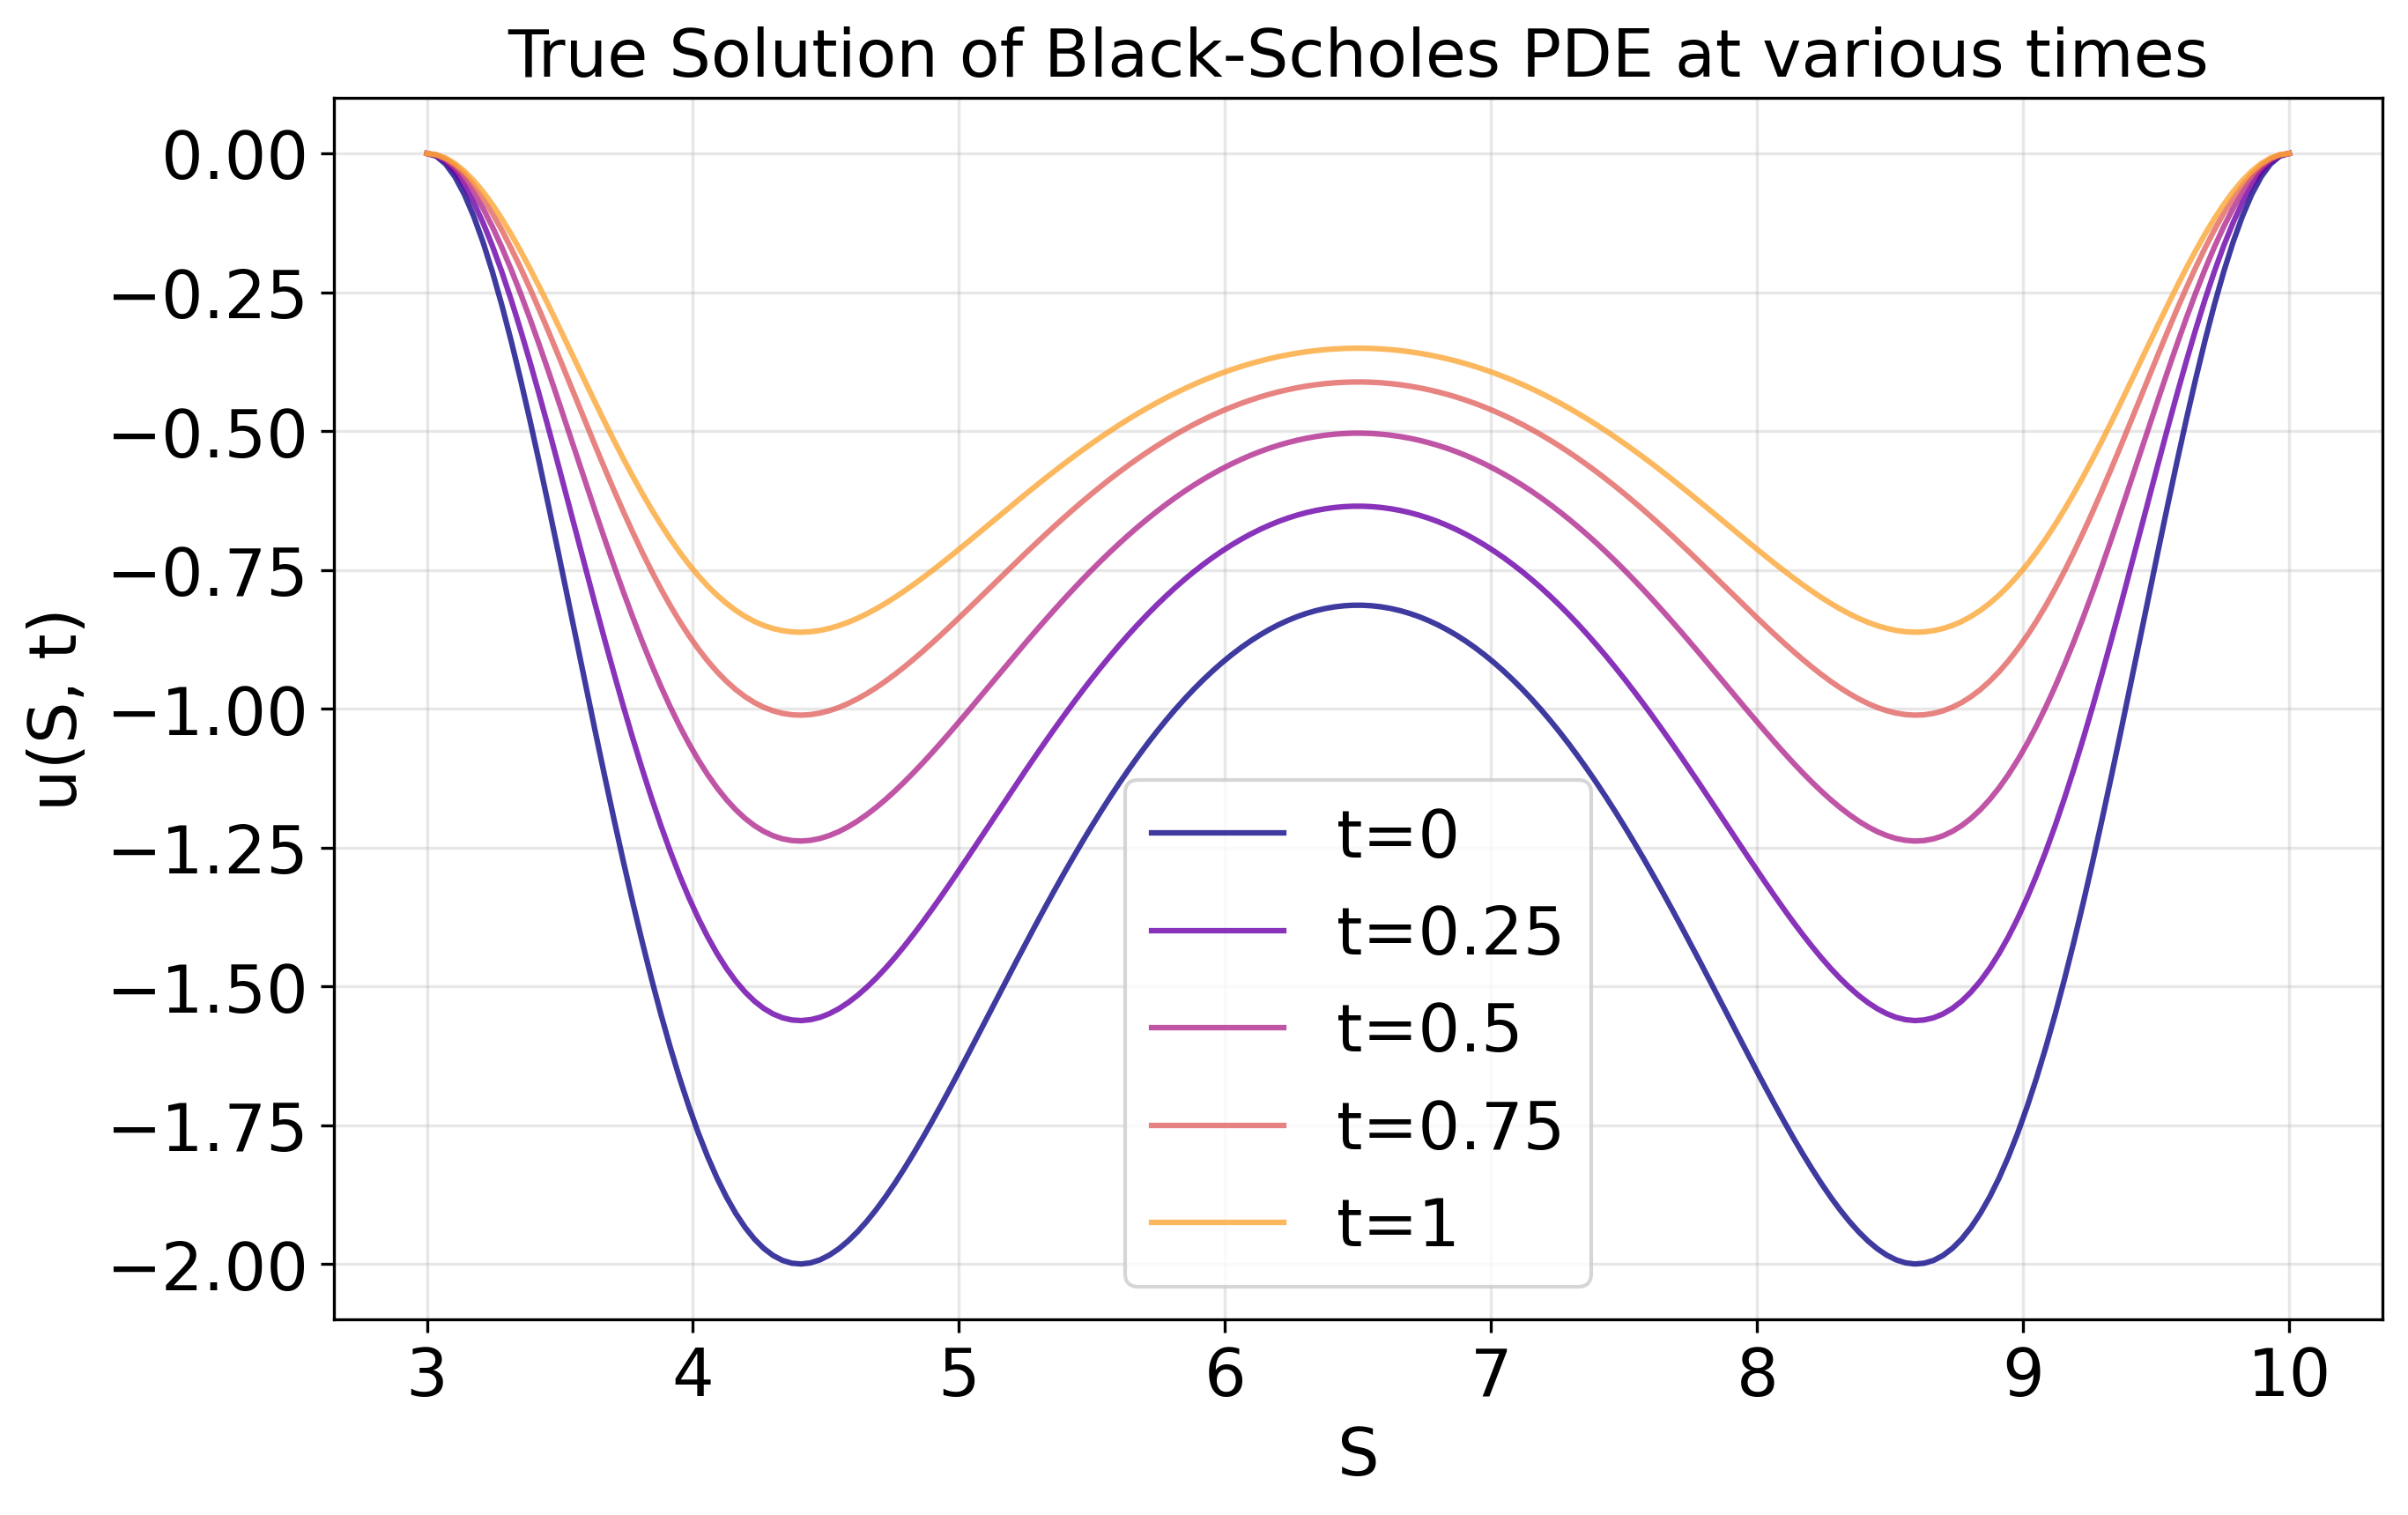
\includegraphics[width=0.75\linewidth]{code/images/true_constructed_cos.png}
    \caption{Analytical solution $u(S,t)$ given by \Cref{eq:constructed_cos} as a function of $S$ for values of $t \in \{0, 0.25, 0.5, 0.75, 1\}$.}
    \label{fig:plot_cos}
\end{figure}

The right-hand side and initial conditions were constructed starting from $u(S,t)$, however the boundary conditions given by \Cref{def:problem} were imposed a priori thus, to make sure \Cref{def:constructed_cos} is a valid solution, we need to verify that $u(S,t)$ agrees with the given boundary conditions.
\begin{lemma}
    The solution $u(S,t)$ proposed in \Cref{eq:constructed_cos} agrees with the boundary conditions stated in \Cref{def:problem}.
\end{lemma}
\begin{proof}
    By constructed we have that $\phi(3)=\phi(10)=0$. Thus $u(10,t)=\left[\cos\left(0\right)-1\right]e^{-\sin(t)} = 0$. Furthermore, the derivative with respect to $S$ of $u(S,t)$ evaluated at $S = 3$ is
    \begin{equation*}
        \dSu(3, t) = \left[-0.4 (6 - 13) \sin(\phi(3))\right]e^{-\sin (t)} = 2.8 \sin(0)e^{-\sin (t)} = 0
    \end{equation*}
    which proves that $u(S,t)$ satisfies the boundary conditions.
\end{proof}

As a initial visual check \Cref{fig:fem_vs_true_cos} illustrates the analytical versus the (interpolated) solution given by the finite element solver. A visual inspection shows that all methods provide a reasonable approximation of the solution. There is, nonetheless, some deviationn with P2 Crank-Nicolson provided the best approximation.

\begin{figure}[!ht]
    \centering
    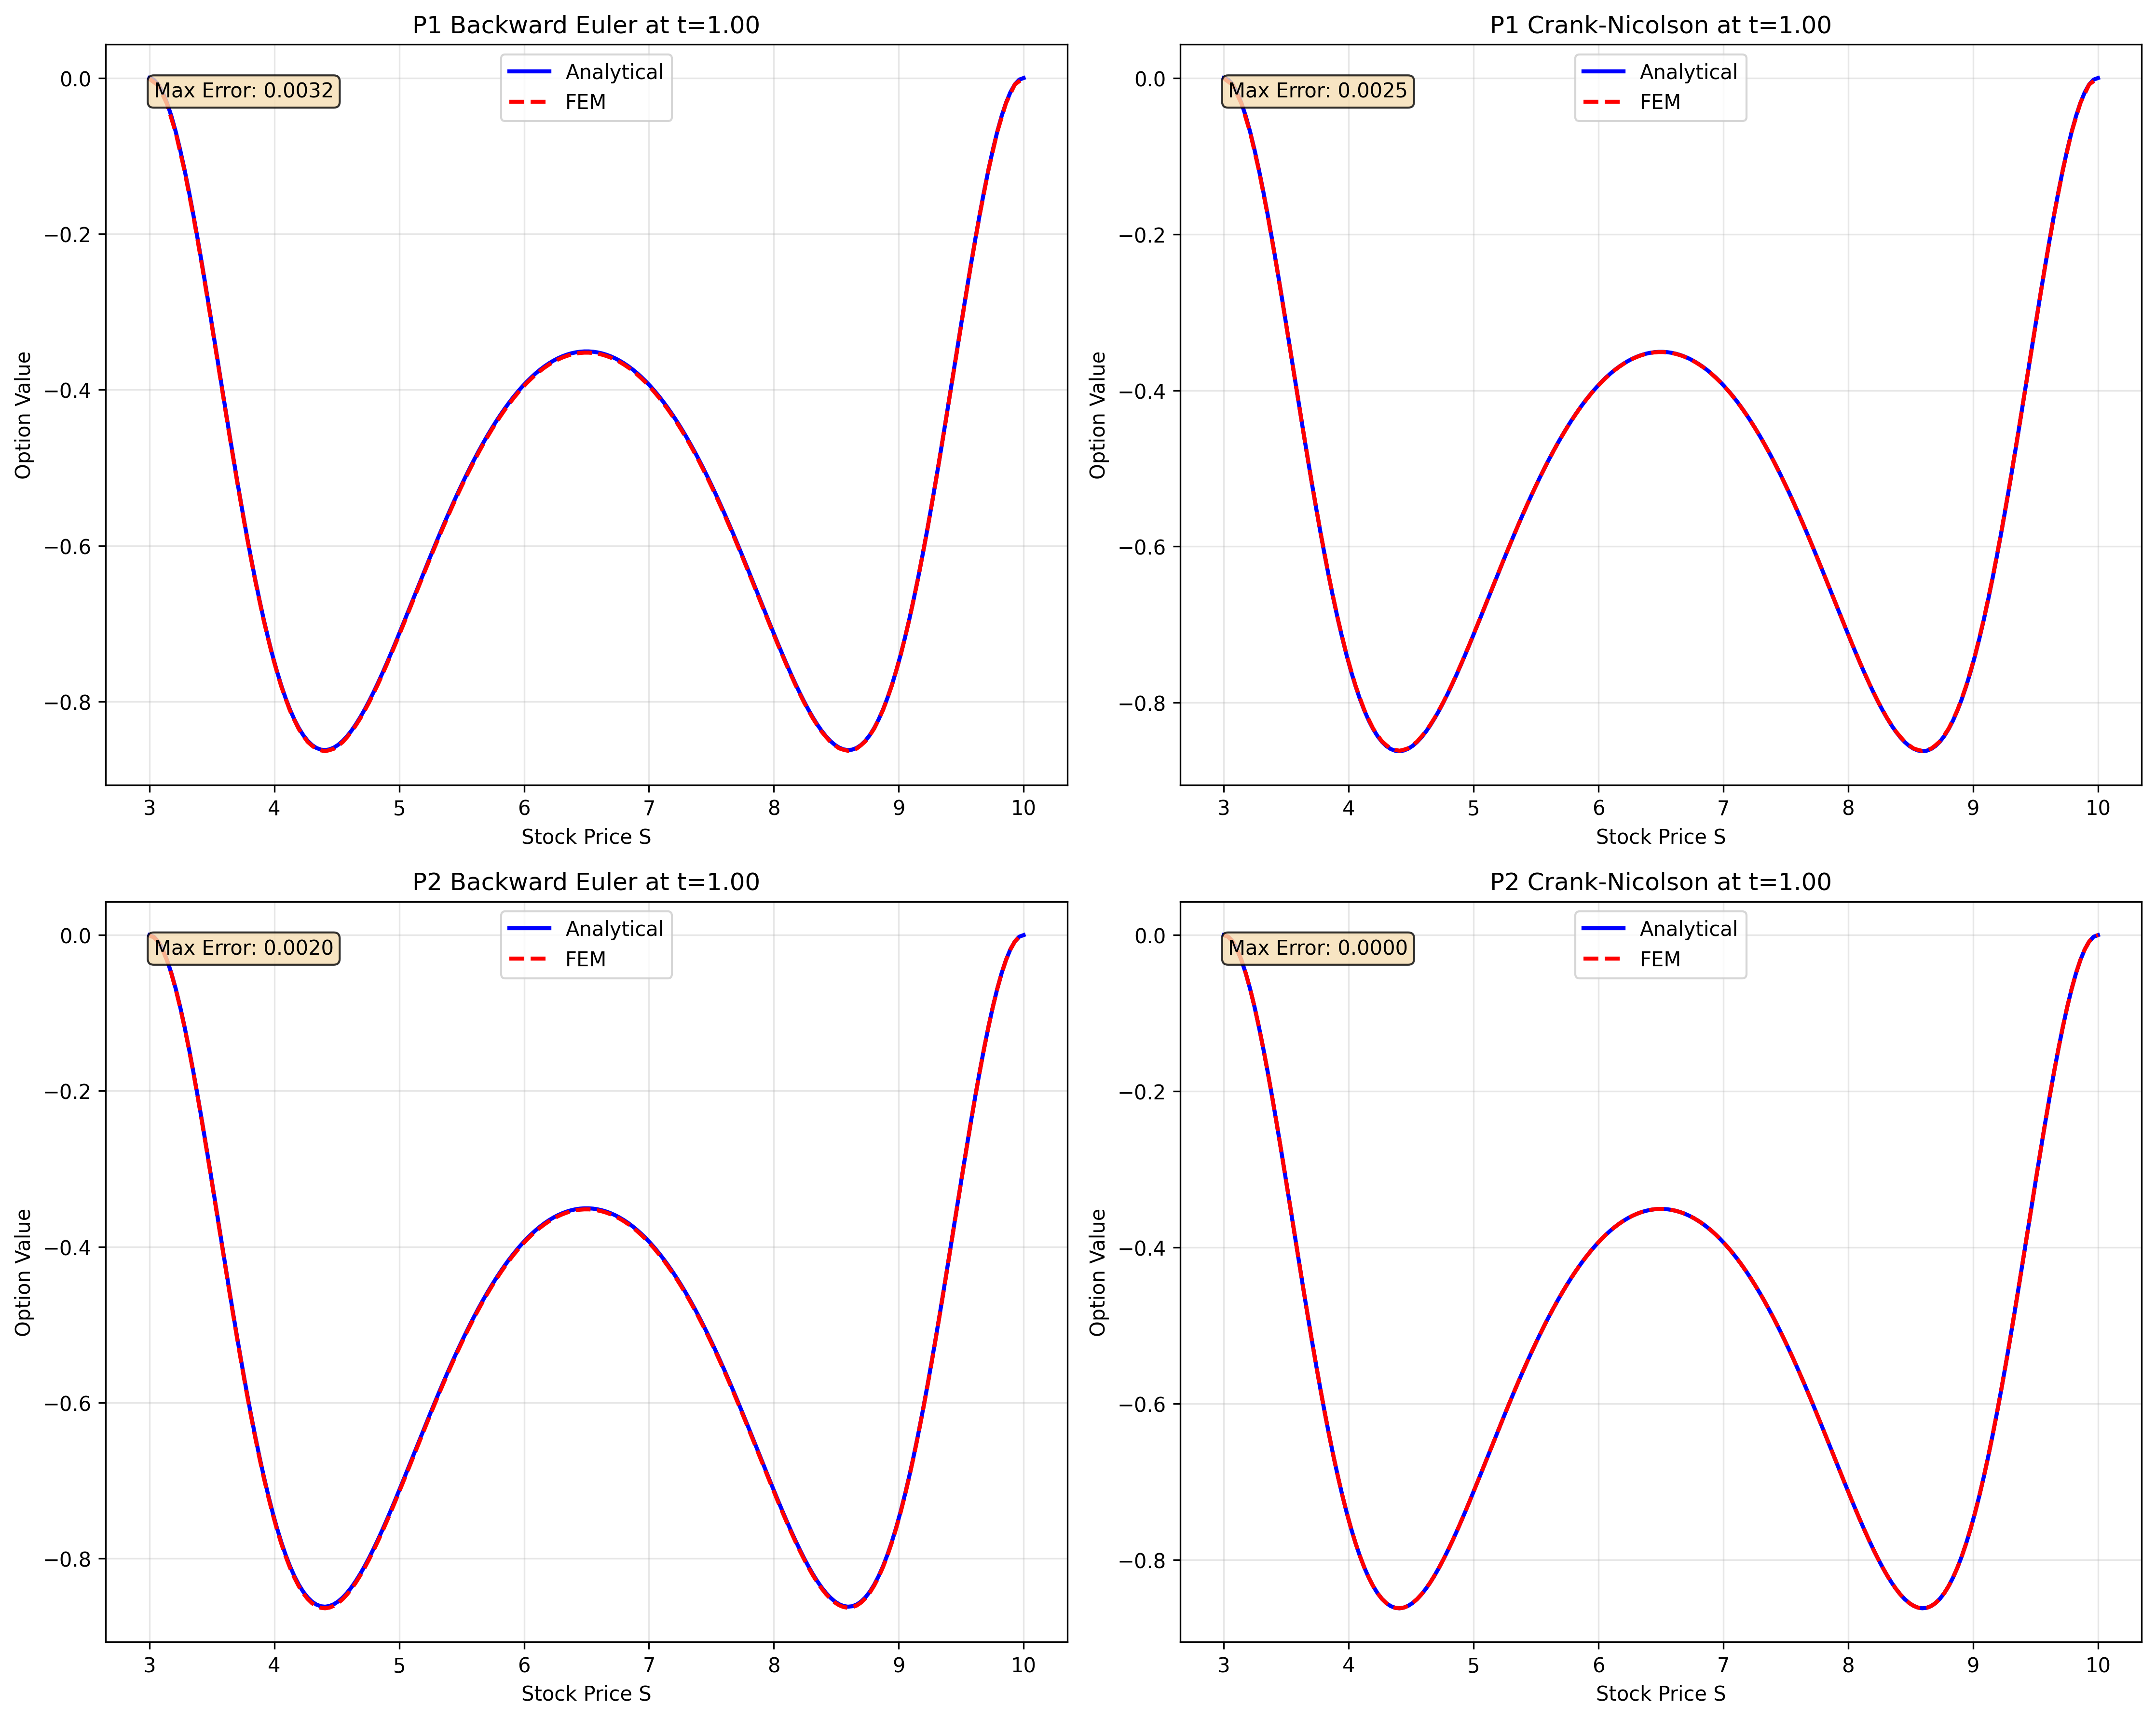
\includegraphics[width=\linewidth]{code/images/fem_vs_analytical_BlackScholesConstructedCos.png}
    \caption{Analytical solution (blue) versus interpolated finite element solution (dashed red) for various methods at time $t=1$ when tasked to solve \Cref{def:constructed_cos}. The PDE was solved with $h =0.07$ and $\Delta t = 3.33 \cdot 10^{-3} $. First and second row correspond to P1 and P2 finite elements respectively. First and second column correspond to backwards Euler and Crank-Nicolson's method respectively. In the top left the maximum errors is presented for all four plots.}
    \label{fig:fem_vs_true_cos}
\end{figure}

\begin{remark}
    To produce \Cref{fig:fem_vs_true_cos} the solution points given by the finite element solver where interpolated using the \href{https://docs.scipy.org/doc/scipy/reference/generated/scipy.interpolate.interp1d.html}{\texttt{scipy.interpolate.interp1d}} function. Nonetheless, all errors throughout the report are computed without interpolation to avoid any interpolation errors contaminating the true errors of the methods.
\end{remark}

% After illustrating that the solver was working the next step was to inspect close the errors. The metrics that were used to quantify errors were the $L^2$ and $L^\infty$ norms. The first step was to understand how these errors evolve over time. The idea is that there might be some errors that accumulate as time evolves. \Cref{fig:error_vs_time_cos} illustrates the $L^2$ and $L^\infty$ errors as a function of time for the methods in question. There is a slight increase in the errors as we get further away from $t=0$, however both norm are plotted in a logarithmic scale and thus the increase of the errors is small.

% \begin{figure}[!ht]
%     \centering
%     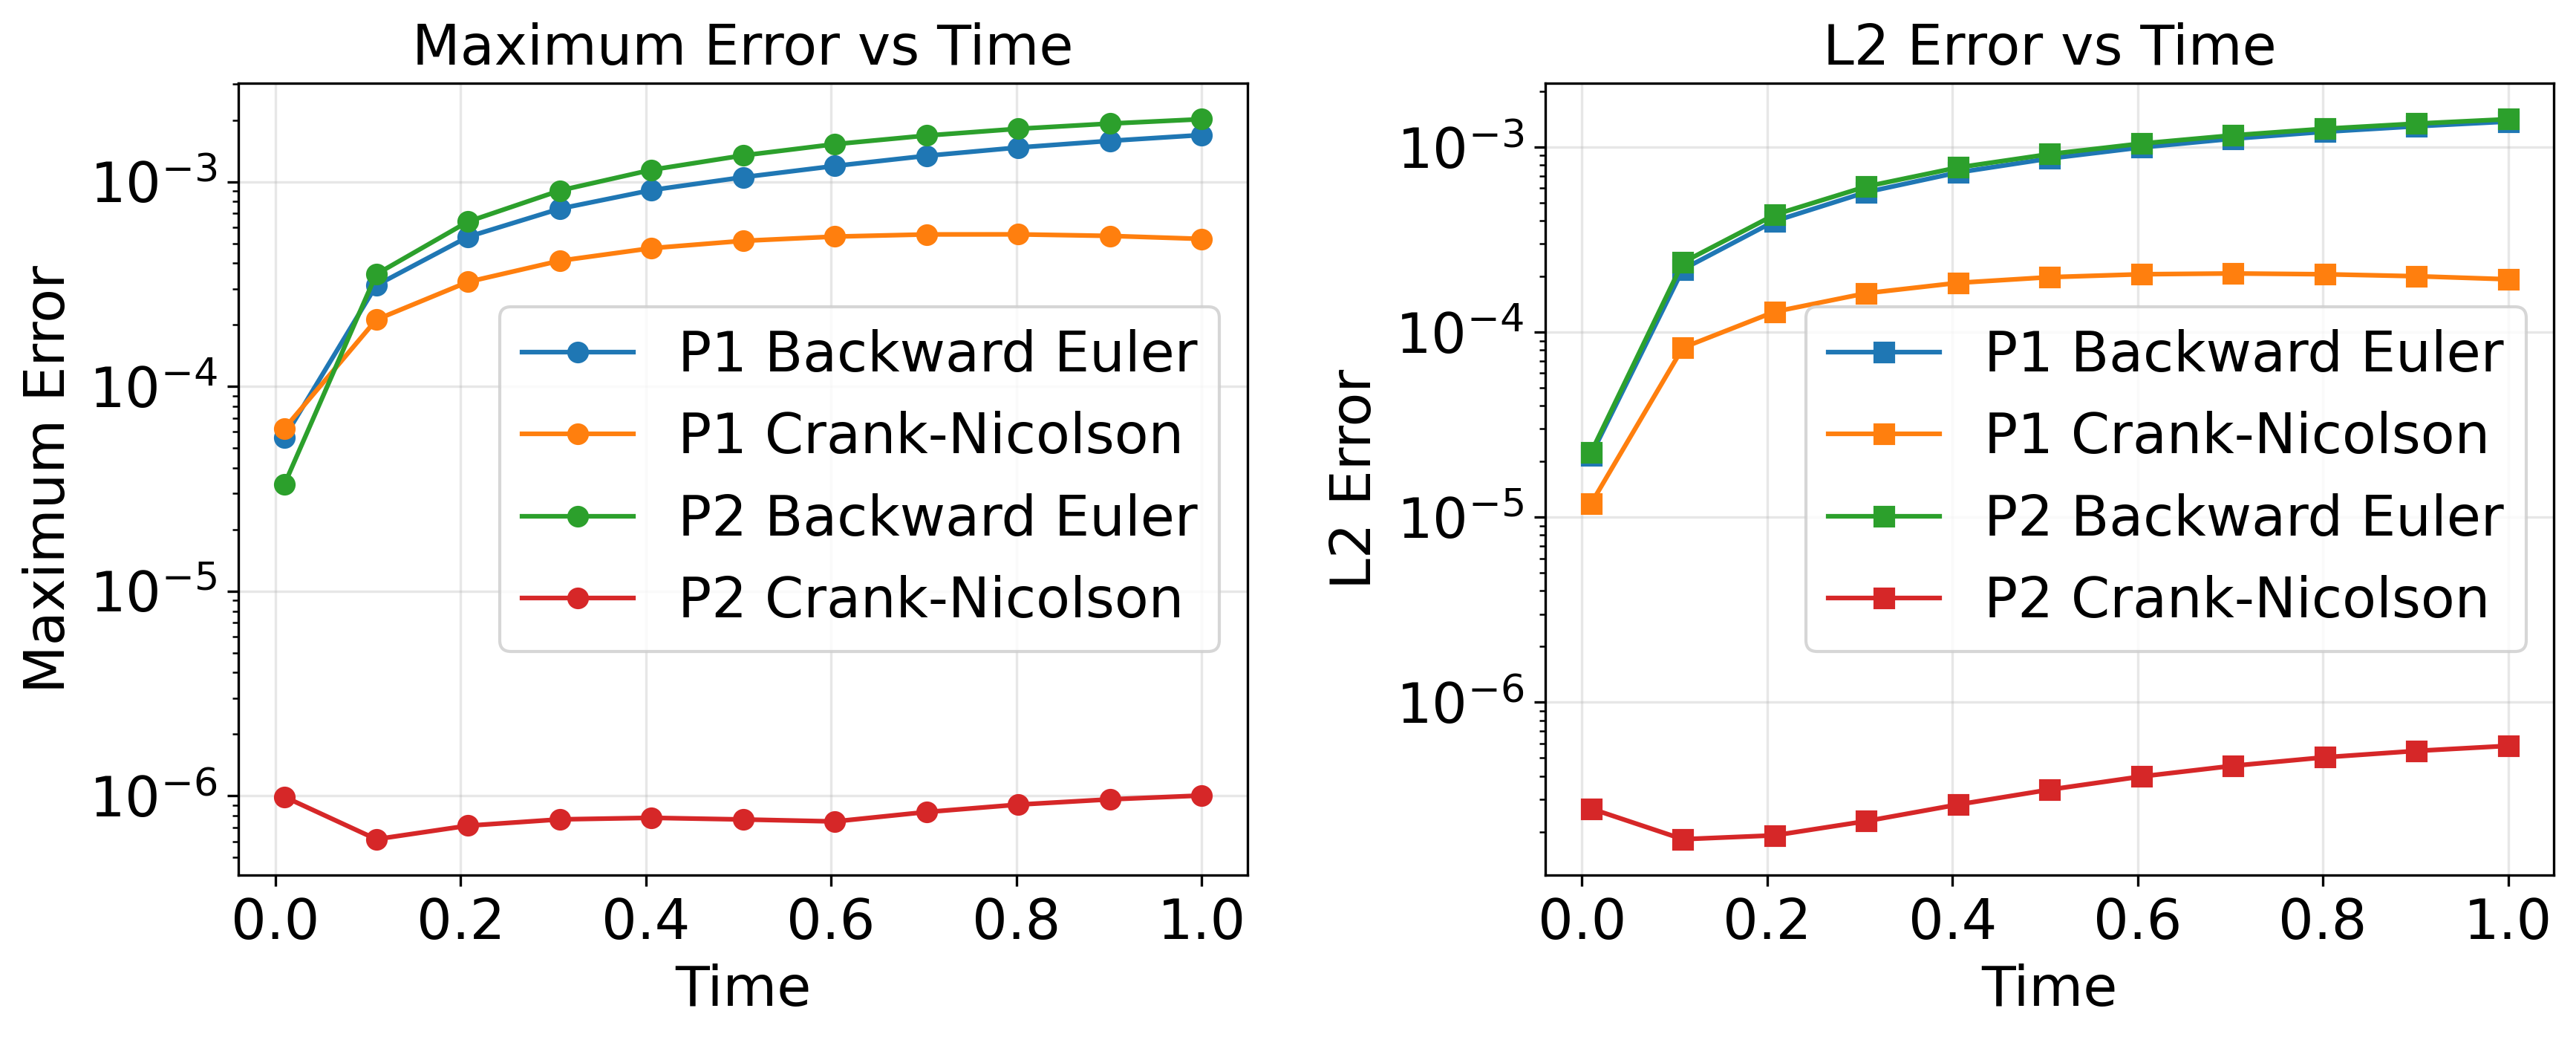
\includegraphics[width=\linewidth]{code/images/error_vs_time_BlackScholesConstructedCos.png}
%     \caption{$L^\infty$ error (left) and $L^2$ error (right) over the full domain of $S \in (3,10)$ as a function of time $t \in [0,1]$ for all four methods. Notice that for the right plot the blue curve is almost identical to the green curve.}
%     \label{fig:error_vs_time_cos}
% \end{figure}

\subsubsection{Convergence study of the constructed solution}
The final experiment on the artificial solution was to perform a convergence study. For the results to be meaningful, it is important that the time discretization error does not dominate. To ensure this, the convergence study was performed using element size $h$ and time interval $\Delta t$ as shown in \Cref{tab:orders}.\\

\begin{table}[h!]
\centering
\begin{tabular}{|c|c|c|}
\hline
 & Backwards Euler & Crank-Nicolson \\
\hline
P1 & $\Delta t \approx h^2$ & $\Delta t \approx h$ \\
\hline
P2 & $\Delta t \approx h^3$ & $\Delta t \approx h^{3/2}$ \\
\hline
\end{tabular}
\caption{Chosen orders of $\Delta t$ as a function of $h$ for the four methods. The order of $\Delta t$ was chosen in such a way that the time discretization error does not dominate when performing the convergence study. The orders of $\Delta t$ were inspired from [1] and [2], and also validated experimentally.}
\label{tab:orders}
\end{table}


Now it is possible to isolate the convergence as a function of the element size $h$. Performing the experiment results in \Cref{fig:conv_cos}. The plot clearly illustrates that both Crank-Nicolson and backwards Euler have a convergence order of $2$ when using P1 finite elements and order $4$ when working with P2 finite elements. 


\begin{figure}[!ht]
    \centering
    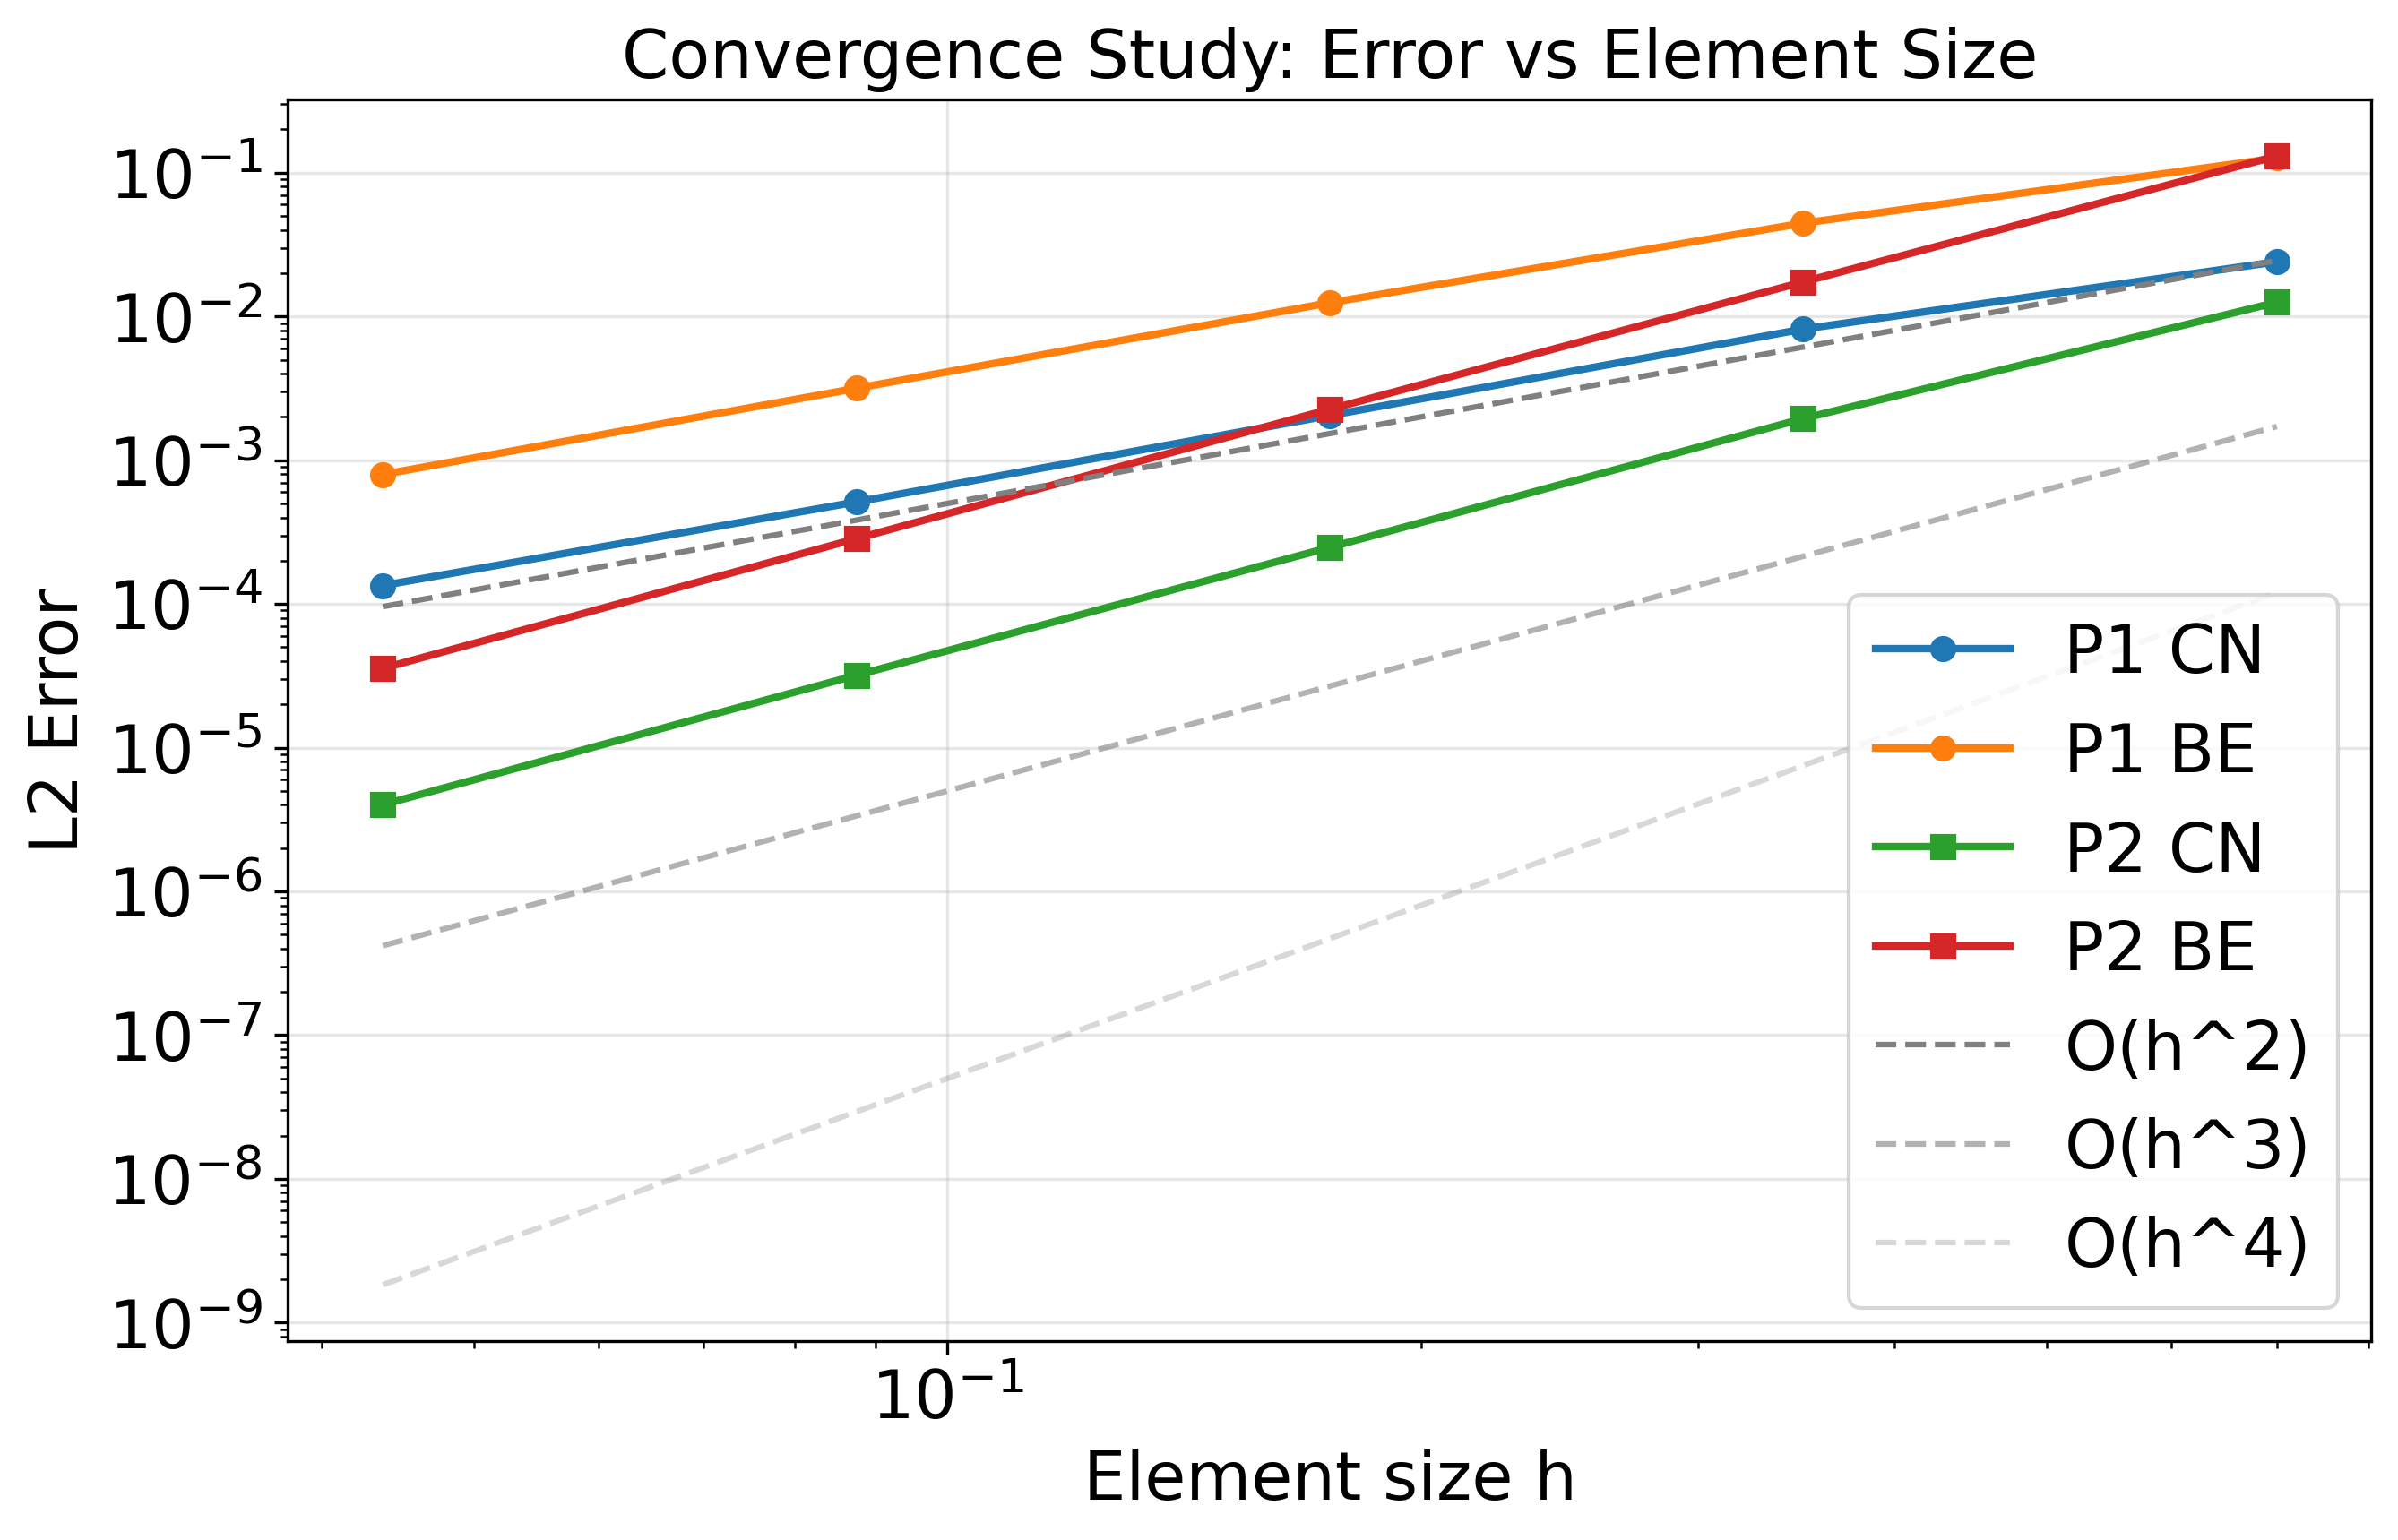
\includegraphics[width=0.75\linewidth]{code/images/convergence_study_BlackScholesConstructedCos.png}
    \caption{Convergence study for all four methods when solving \Cref{def:constructed_cos}.}
    \label{fig:conv_cos}
\end{figure}

\subsection{True solution}\label{sec:true_sol}
With the results presented in the previous section, the next step is to perform the same study on the analytical solution of \Cref{def:problem}. The parameters are chosen as: $S_{min}=0, S_{max}=300, K=100, r=0.04, \sigma =0.2, $ and $T = 5$. To begin \Cref{fig:fem_vs_true_true} illustrate the analytical solution when compared to the interpolated solution of the finite element solver. Visually it is clear that all the methods manage to capture the analytical solution. It is, however, important to point out that the maximum errors are indeed large than before. This will also be evident in the convergence study. 

\begin{figure}[!ht]
    \centering
    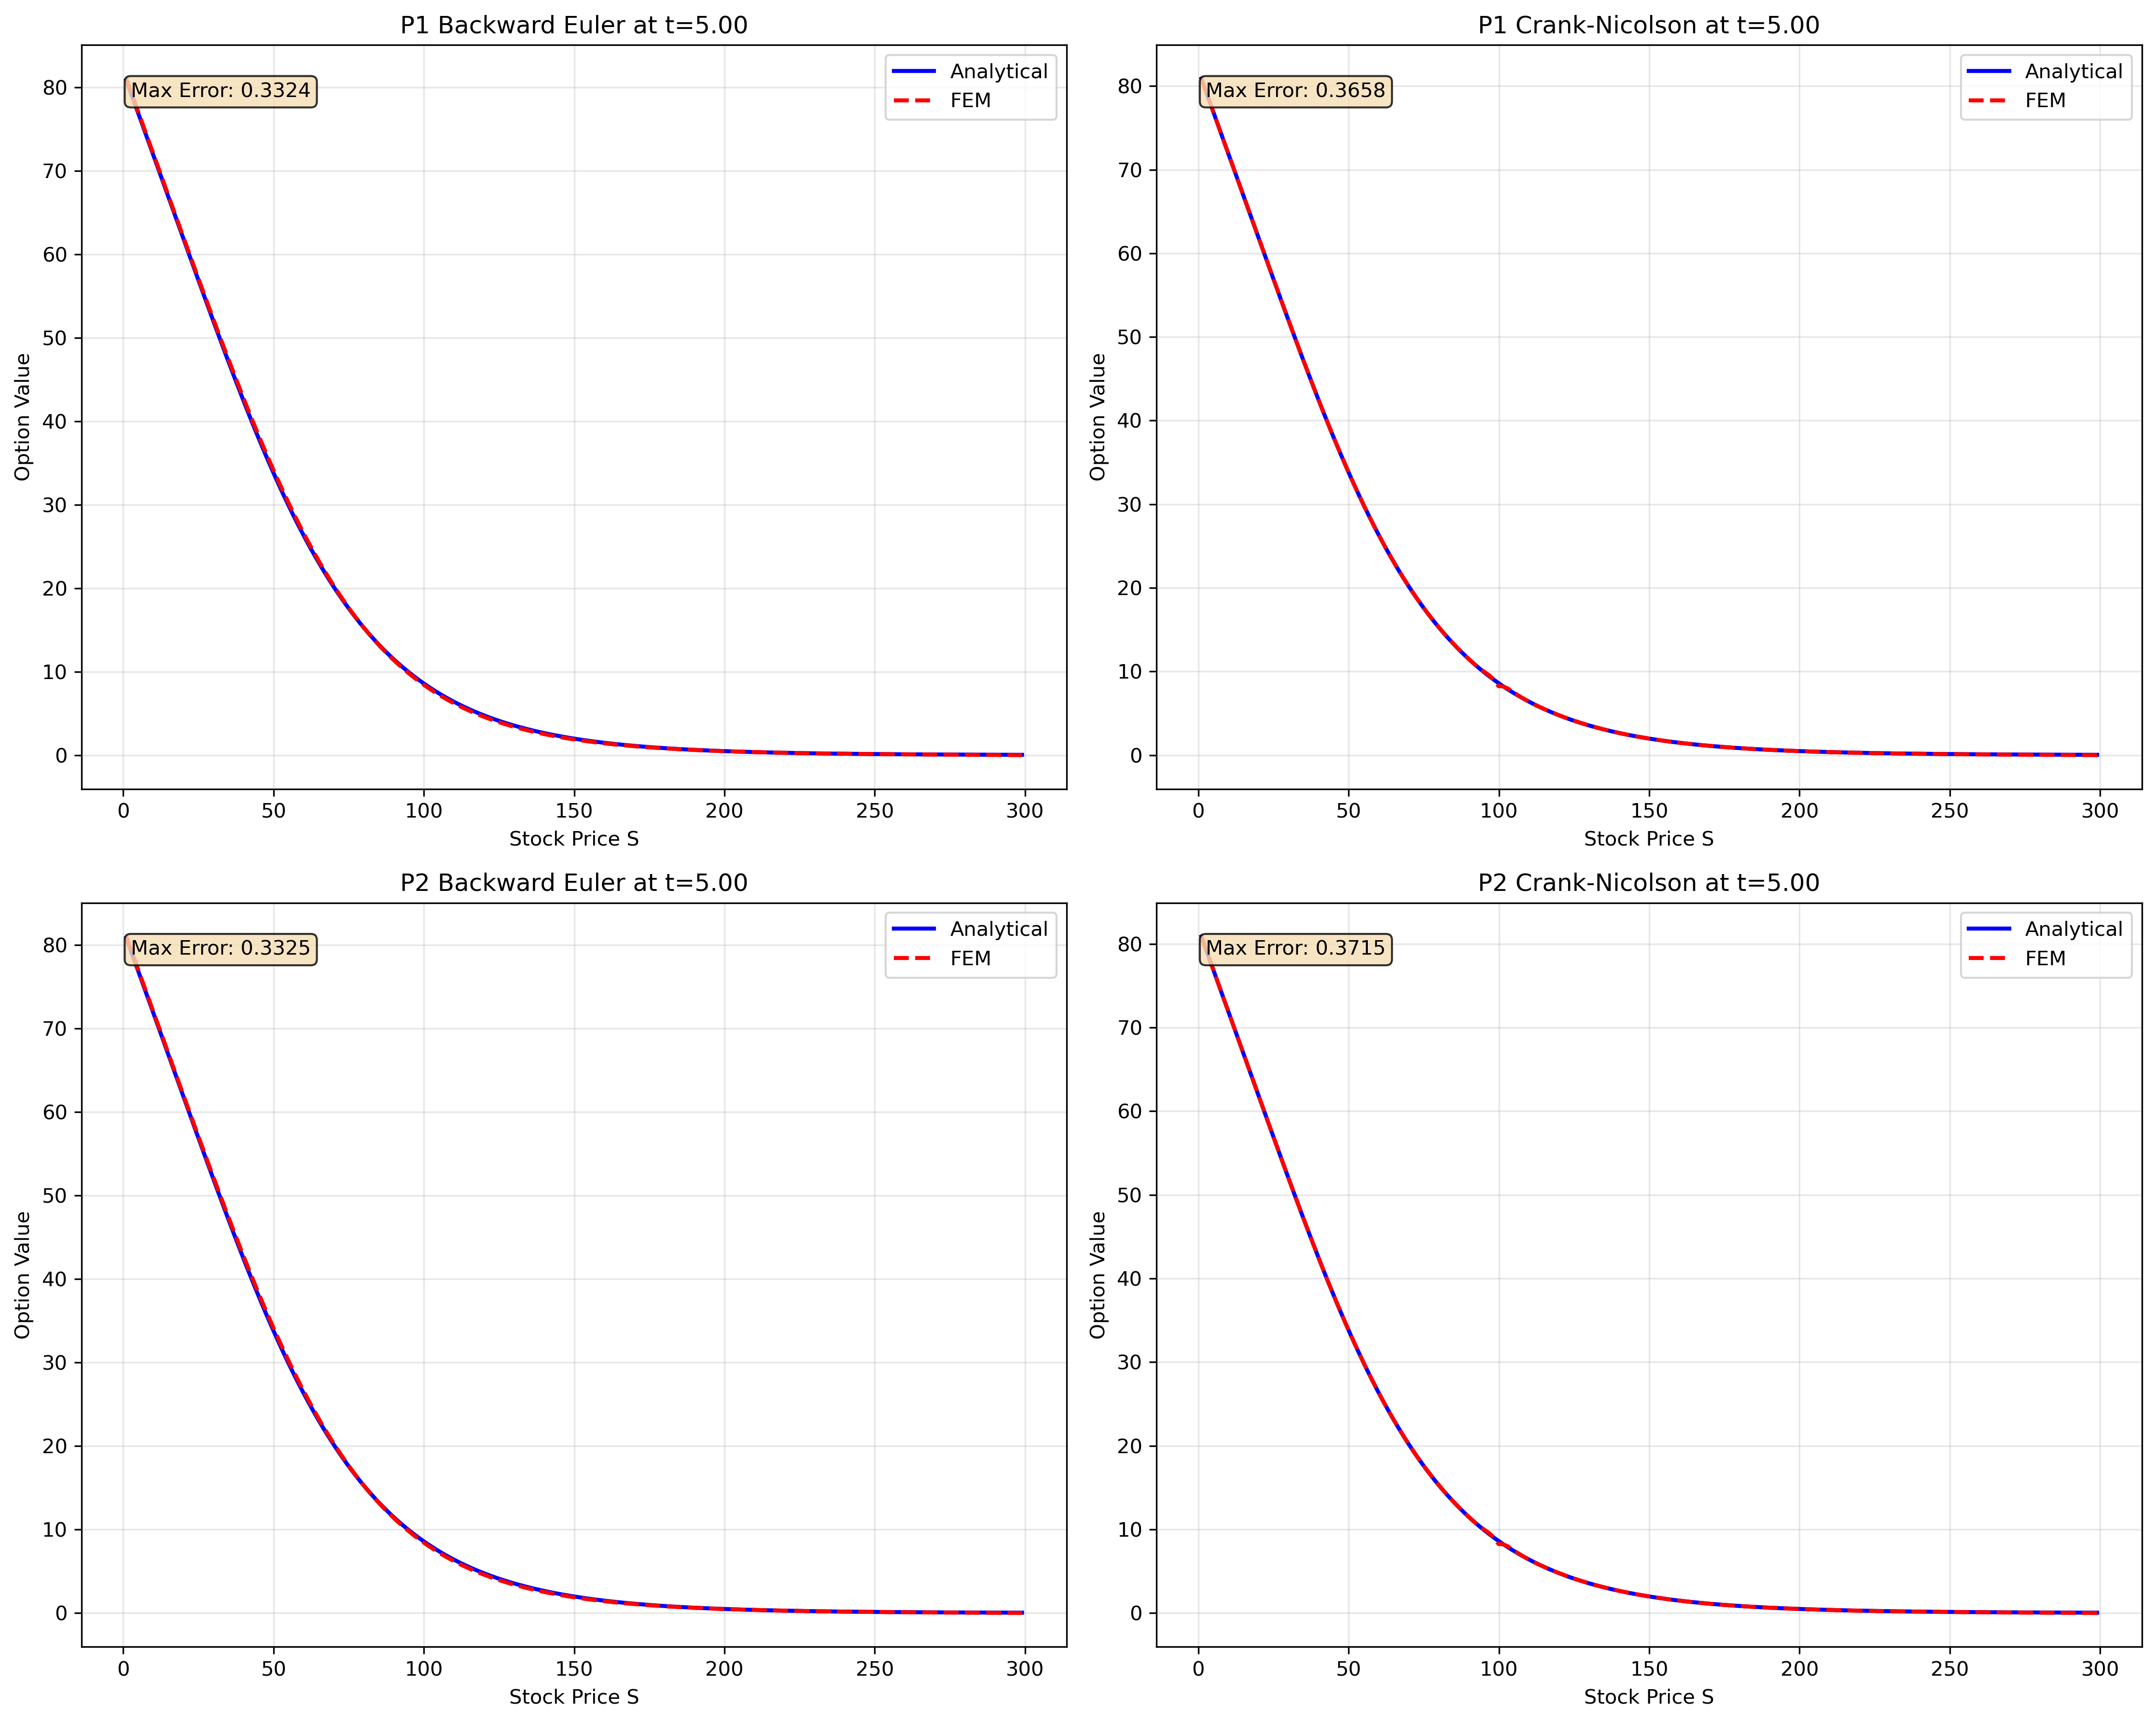
\includegraphics[width=\linewidth]{code/images/fem_vs_analytical_BlackScholesTrue.png}
    \caption{Analytical solution (blue) versus interpolated finite element solution (dashed red) for various methods at time $t=1$ when tasked to solve \Cref{def:problem}. The PDE was solved with $h =0.5$ and $\Delta t = 0.5 $. First and second row correspond to P1 and P2 finite elements respectively. First and second column correspond to backwards Euler and Crank-Nicolson's method respectively. In the top left the maximum errors is presented for all four plots.}
    \label{fig:fem_vs_true_true}
\end{figure}

\subsubsection{Convergence study of the true solution}
Recalling \Cref{tab:orders}, in this section a very similar convergence study is performed. The results are shown in \Cref{fig:conv_true}. 
\begin{figure}[!ht]
    \centering
    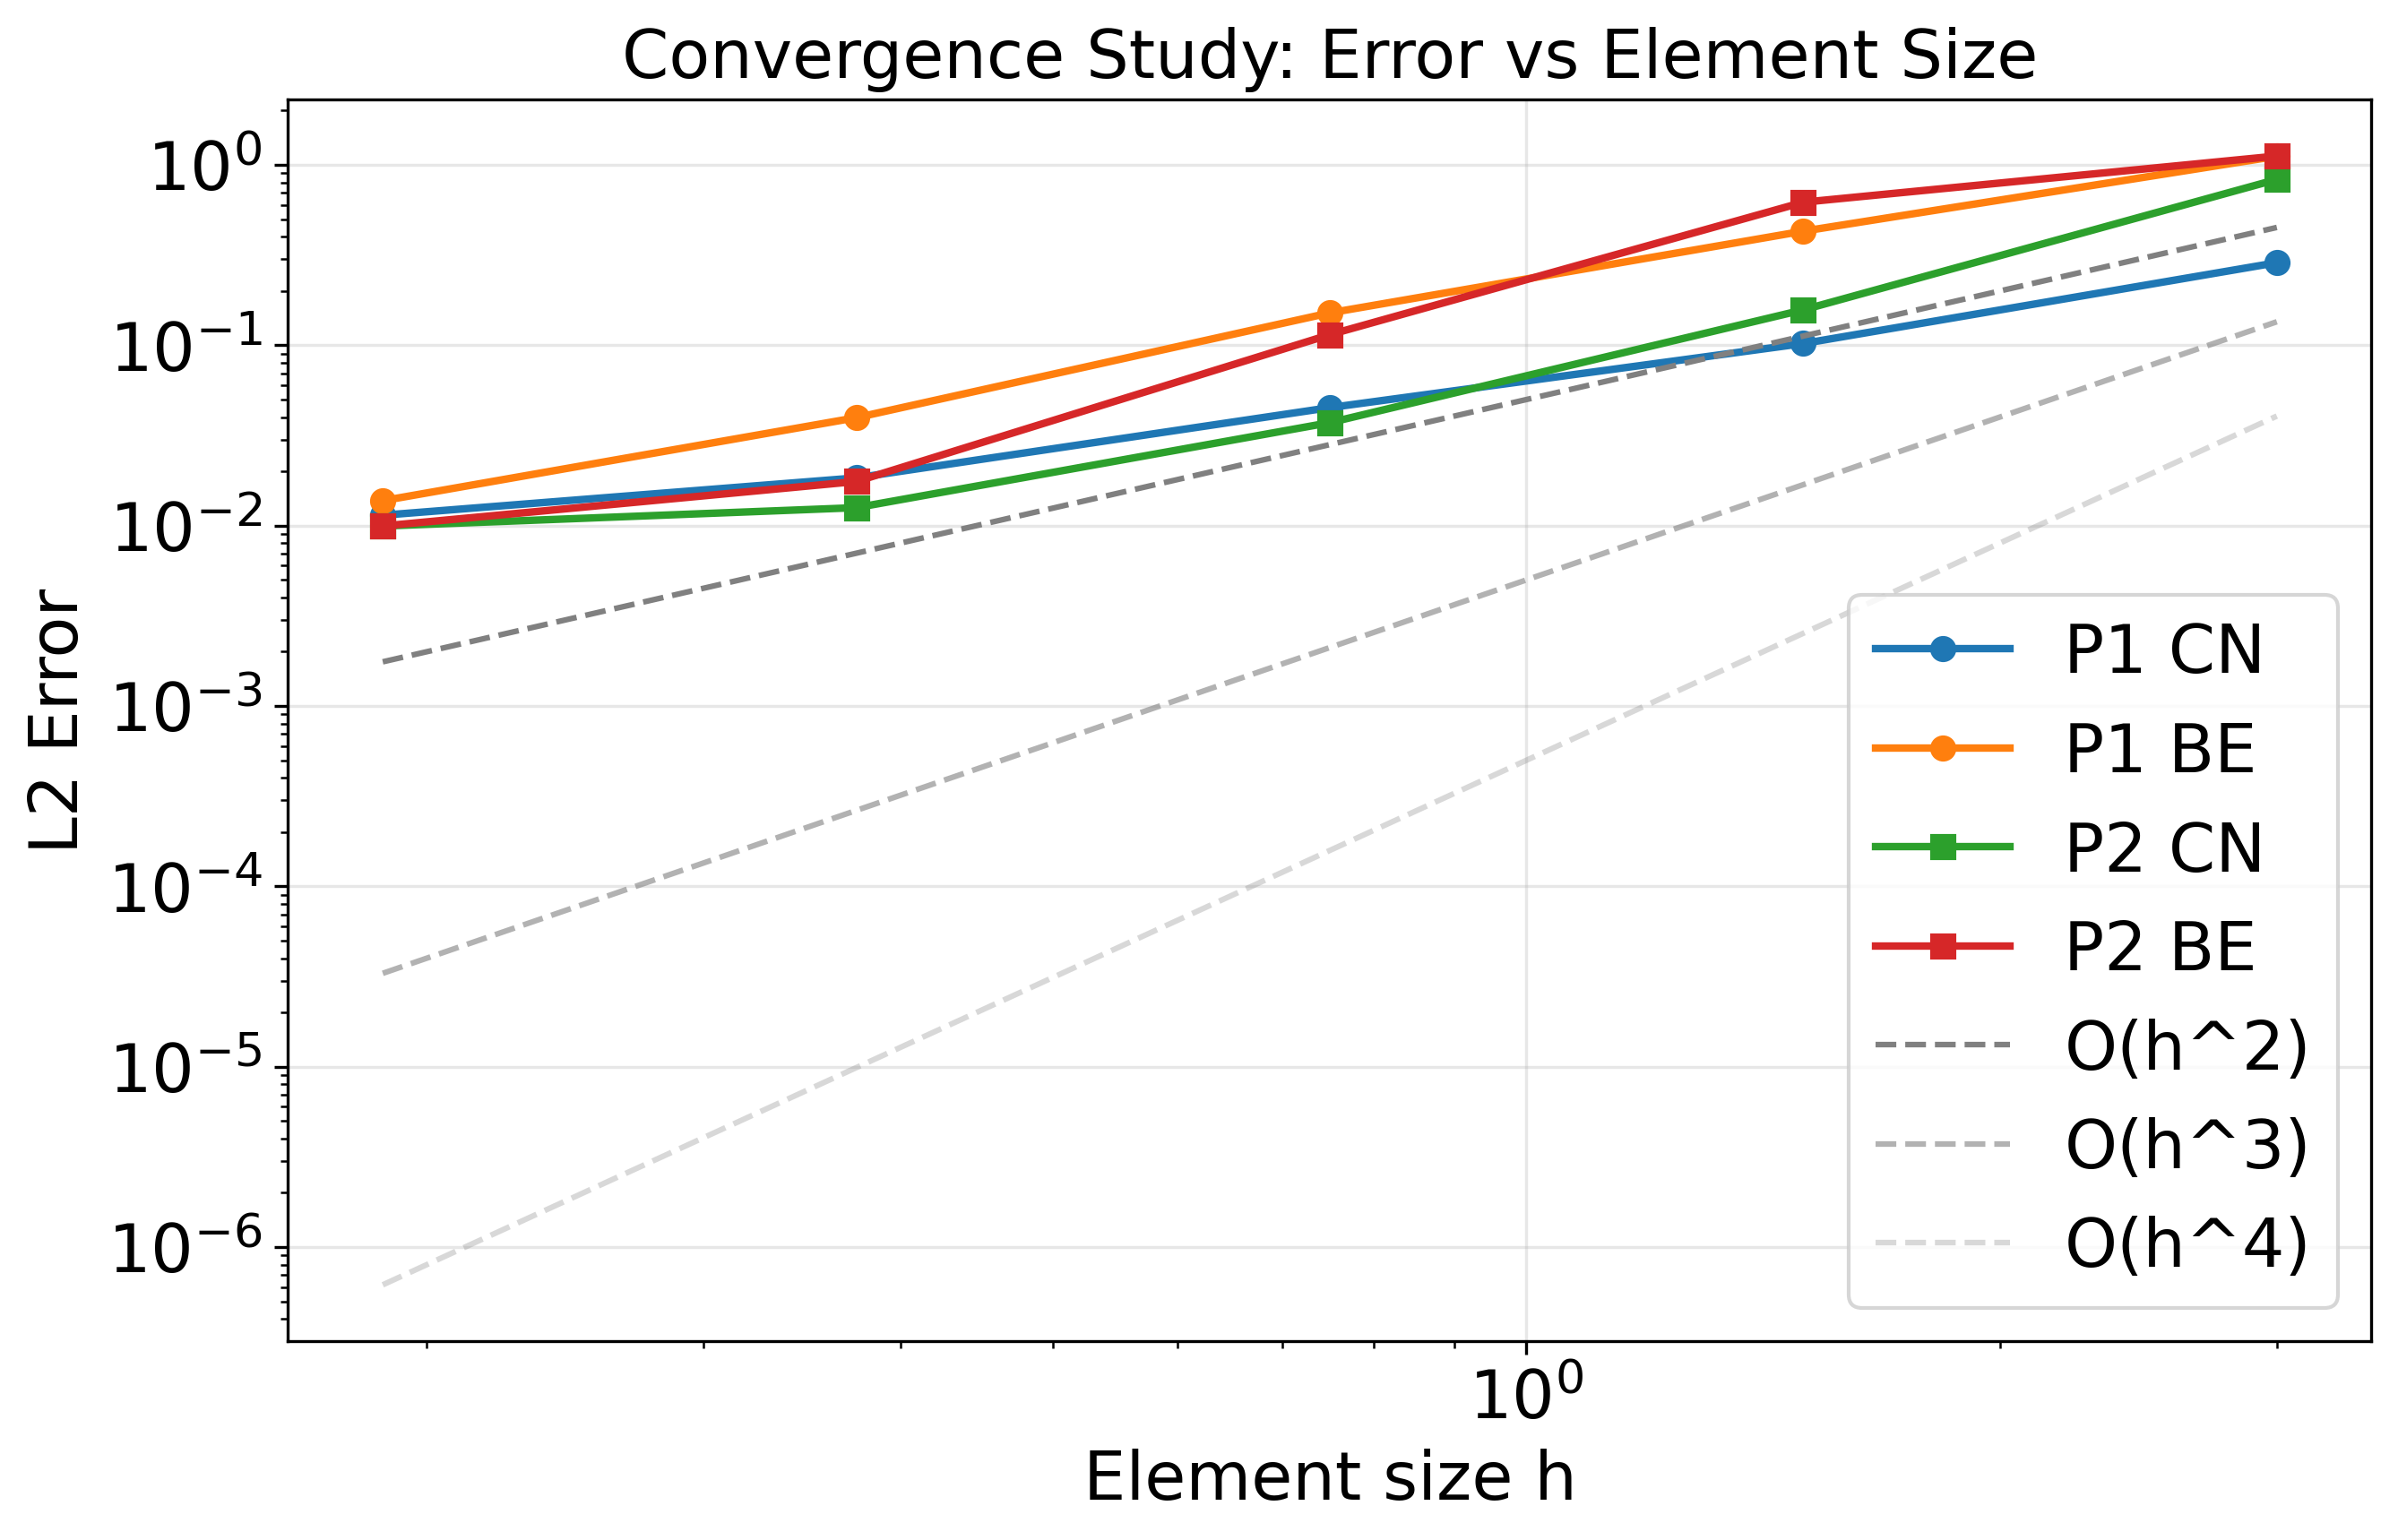
\includegraphics[width=0.75\linewidth]{code/images/convergence_study_BlackScholesTrue.png}
    \caption{Convergence study for all four methods when solving \Cref{def:constructed_cos}.}
    \label{fig:conv_true}
\end{figure}

The first striking observation is that the solver struggles a lot more to solve this problem than \Cref{def:constructed_cos}. There are many reasons why this might be. First the space $\Omega$ and the final time $T$ are much large, leaving way for numerical errors to appear and propagate. Secondly, and more importantly, if the lack of smoothness in the initial condition of \Cref{def:problem}. Indeed this initial has a problematic point at $S=K$. This leading to an overall suboptimal outcome of the finite element solver. There are some possible solutions to this problem. The first candidate is to use higher order finite elements. While being costly, this is likely to help by providing a better approximation and reducing any errors when using P1 or P2 elements. Indeed, one pattern visible in \Cref{fig:conv_true} is that for a given $h$ the P2 finite elments


\newpage
\section*{References}
\begin{itemize}
    \item[] [1] Brenner, Susanne, and L. Ridgway Scott. \textit{The Mathematical Theory of Finite Element Methods}. 1st ed. vol. 15. New York, NY: Springer, 1994.
    \item[] [2] Achdou, Y. and Pironneau, O., 2005. \textit{Computational methods for option pricing} (Vol. 30). Siam
\end{itemize}


\appendix
\section{Green's formulas}
In this appendix we present some useful formulas.

% \begin{thm}[Gauss--Ostrogradsky's formula]\label{thm:div}
% Let $\Omega \subset \mathbb{R}^n$ be a bounded set with $\partial\Omega \subset C^1$. For $u \in C^1(\bar{\Omega})$,
% \[
% \int_\Omega u_{x_i}(x)\,dx = \int_{\partial\Omega} u(y)\nu_i(y)\,dS(y), \qquad i = 1, \cdots, n.
% \]
% \end{thm}

\begin{thm}[Integration by parts formula] \label{thm:by_parts}
Let $\Omega \subset \mathbb{R}^n$ be a bounded set with $\partial\Omega \subset C^1$. For $u, v \in C^1(\bar{\Omega})$,
\[
\int_\Omega u_{x_i}(x)v(x)\,dx = -\int_\Omega u(x)v_{x_i}(x)\,dx + \int_{\partial\Omega} u(y)v(y)\nu_i(y)\,dS(y), \qquad i = 1, \cdots, n.
\]
or, in vectorial form,
\[
\int_\Omega \nabla u(x)v(x)\,dx = -\int_\Omega u(x)\nabla v(x)\,dx + \int_{\partial\Omega} u(y)v(y)\nu(y)\,dS(y)
\]
\end{thm}

% \begin{thm}[Green’s identities] \label{thm:green_id}
% Let $\Omega \subset \mathbb{R}^n$ be a bounded set with $\partial\Omega \subset C^1$. For $u, v \in C^2(\bar{\Omega})$,
% \[
% \int_\Omega \Delta u\,dx = \int_{\partial\Omega} \partial_\nu u\,dS,
% \]
% with $\partial_\nu u = \nabla u \cdot \nu$ being the normal derivative of $u$, and
% \[
% \int_\Omega v \Delta u\,dx = -\int_\Omega \nabla u \cdot \nabla v\,dx + \int_{\partial\Omega} v\partial_\nu u\,dS = \int_\Omega u\Delta v\,dx + \int_{\partial\Omega} (v \partial_\nu u - u \partial_\nu v)\,dS.
% \]
% \end{thm}

All previous identities are valid also if the boundary $\partial\Omega$ is only Lipschitz continuous (since Lipschitz functions are differentiable everywhere but a set of points of Lebesgue measure zero).


\begin{lemma}[Lax-Milgram Lemma]\label{lemma:lax_mil}
    Given a Hilbert space $V$ and a bilinear form $b(\cdot, \cdot)$ on $V$ such that
    \begin{align*}
        & b(u,v) \leq M \| u\|_V \| v\|_V \quad \text{ (Continuity) }\\
        &b(u,u) \geq \beta \| u\|_V^2 \qquad \hspace{6mm} \text{ (Coercivity) }
    \end{align*}
    for some $M,\beta>0$ then, given a bounded functional $F$ on $V$, the problem
    \begin{equation*}
        b(u,v) = F(v)
    \end{equation*}
    admits a unique solution. Moreover, $\| u\|_V \leq \frac{1}{\beta} \| F\|_{V'}$.
\end{lemma}

\section{Additional constructed solution}\label{appendix:extra}

    



\end{document}